\problemname{Rullebånd}

På lufthavnen skal du igennem en lang gang med rullende fortove for at komme til bagageudleveringen.
Gangen er $M$ meter lang, og du står i begyndelsen af den og overvejer, hvor hurtigt du kan komme frem til bagageudleveringen. 
Der er $N$ rullende fortove i gangen.
Hvert rullende fortov består af et bånd, der begynder på en vis afstand fra begyndelsen af gangen, slutter på en vis afstand fra begyndelsen af gangen og tager en vis tid at køre langs.
Alle bånd går i gangens retning, man kan kun stige på i begyndelsen og stige af i slutningen af båndet.
Når holdet ikke er på et rullende fortov, tager det $g$~sekunder at gå $1$~meter.
Gangen og rullebåndende er så smalle, at I kan nøjes med at se på den tid, det tager at flytte sig parallelt med gangen.
Det betyder, at hvis et bånd slutter i samme afstand fra gangens begyndelse som et andet begynder, så tager det ingen tid at gå fra det ene bånd til det andet.
Hvad er den hurtigste tid man kan komme til enden af gangen?

Læg mærke til, at det sommetider kan betale sig at gå »baglæns« i gangen, for at kommet til et hurtigt rullende fortov som tager holdet langt fremad.
Ingen af de rullende fortove kører baglæns.

\section*{Indlæsning}
Første linje indeholder tre heltal $N$, $M$, $g$ ($1 \le N \le 2 \times 10^5$, $2 \le M \le 2 \times 10^5$, $1 \le g \le 100$):
antallet af rullende fortov, gangens længde i meter og holdets ganghastighed i sekunder per meter.
Hver af de følgende $N$ linjer beskriver et rullende fortov og indeholder hver 3 heltal: $s_i, e_i$ og $t_i$
($1\leq s_i,e_i\leq M,1\leq t_i\leq100$).
Her er $s_i$  antallet meter fra begyndelsen af gangen til båndets begyndelse, $e_i$ antallet af meter fra begyndelsen af gangen til båndets slutning og $t_i$ antallet af sekunder, det tager at køre båndet fra begyndelsen til slutningen.

\section*{Udskrift}
Udskriv en linje med et heltal: det mindste antal sekunder det tager at komme gennem gangen.

\section*{Pointgivning}
Din løsning bliver kørt på et antal testfaldsgrupper.
For at få point for en gruppe skal du klare alle testfald i gruppen.

\noindent
\begin{tabular}{ l  l  l }
Gruppe & Point & Begrænsninger \\ \hline
1     & 8          &  $N,M \le 10$ og man behøver aldrig at gå bagud\\ 
2     & 13         &  $N,M \le 1000$ og man behøver aldrig at gå bagud\\ 
3     & 40         &  $N,M \le 10^5$ og man behøver aldrig at gå bagud\\ 
4     & 15         &  $N,M \le 1000$. \\ 
5     & 24         &  $N,M \le 10^5$. 
\end{tabular}

\section*{Forklaring af eksemplerne}

\begin{figure}[h]
	\centering
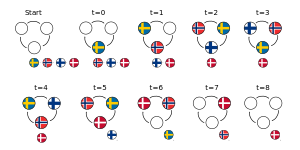
\includegraphics[width=0.7\textwidth]{sample1}
\caption{Eksempel 1}
\end{figure}
I eksempel 1 tager det 2 sekunder at gå en meter, når holdet ikke er på noget rullende fortov.
Den hurtigste måde at komme igennem gangen er at gå til 5-sekundersbåndet, køre med det, derfra gå videre til 2-sekundersbåndet og køre med det.
Sammenlagt tager dette $4+5+2+2=13$ sekunder.



\begin{figure}[h]
	\centering

\includegraphics[width=0.7\textwidth]{sample2}
\caption{Eksempel 2}
\end{figure}
I eksempel 2 tager det i stedet 5 sekunder at gå en meter, når holdet ikke er på noget rullende fortov.
Den hurtigste måde at komme igennem gangen er at gå til 8-sekundersbåndet, køre med det, gå 1~meter tilbage, tage 2-sekundersbåndet og gå den sidste meter.
Den sammenlagte tid er $5+8+5+2+5=25$ sekunder.
